\documentclass[twoside]{book}

% Packages required by doxygen
\usepackage{fixltx2e}
\usepackage{calc}
\usepackage{doxygen}
\usepackage[export]{adjustbox} % also loads graphicx
\usepackage{graphicx}
\usepackage[utf8]{inputenc}
\usepackage{makeidx}
\usepackage{multicol}
\usepackage{multirow}
\PassOptionsToPackage{warn}{textcomp}
\usepackage{textcomp}
\usepackage[nointegrals]{wasysym}
\usepackage[table]{xcolor}

% Font selection
\usepackage[T1]{fontenc}
\usepackage[scaled=.90]{helvet}
\usepackage{courier}
\usepackage{amssymb}
\usepackage{sectsty}
\renewcommand{\familydefault}{\sfdefault}
\allsectionsfont{%
  \fontseries{bc}\selectfont%
  \color{darkgray}%
}
\renewcommand{\DoxyLabelFont}{%
  \fontseries{bc}\selectfont%
  \color{darkgray}%
}
\newcommand{\+}{\discretionary{\mbox{\scriptsize$\hookleftarrow$}}{}{}}

% Page & text layout
\usepackage{geometry}
\geometry{%
  a4paper,%
  top=2.5cm,%
  bottom=2.5cm,%
  left=2.5cm,%
  right=2.5cm%
}
\tolerance=750
\hfuzz=15pt
\hbadness=750
\setlength{\emergencystretch}{15pt}
\setlength{\parindent}{0cm}
\setlength{\parskip}{3ex plus 2ex minus 2ex}
\makeatletter
\renewcommand{\paragraph}{%
  \@startsection{paragraph}{4}{0ex}{-1.0ex}{1.0ex}{%
    \normalfont\normalsize\bfseries\SS@parafont%
  }%
}
\renewcommand{\subparagraph}{%
  \@startsection{subparagraph}{5}{0ex}{-1.0ex}{1.0ex}{%
    \normalfont\normalsize\bfseries\SS@subparafont%
  }%
}
\makeatother

% Headers & footers
\usepackage{fancyhdr}
\pagestyle{fancyplain}
\fancyhead[LE]{\fancyplain{}{\bfseries\thepage}}
\fancyhead[CE]{\fancyplain{}{}}
\fancyhead[RE]{\fancyplain{}{\bfseries\leftmark}}
\fancyhead[LO]{\fancyplain{}{\bfseries\rightmark}}
\fancyhead[CO]{\fancyplain{}{}}
\fancyhead[RO]{\fancyplain{}{\bfseries\thepage}}
\fancyfoot[LE]{\fancyplain{}{}}
\fancyfoot[CE]{\fancyplain{}{}}
\fancyfoot[RE]{\fancyplain{}{\bfseries\scriptsize Generated by Doxygen }}
\fancyfoot[LO]{\fancyplain{}{\bfseries\scriptsize Generated by Doxygen }}
\fancyfoot[CO]{\fancyplain{}{}}
\fancyfoot[RO]{\fancyplain{}{}}
\renewcommand{\footrulewidth}{0.4pt}
\renewcommand{\chaptermark}[1]{%
  \markboth{#1}{}%
}
\renewcommand{\sectionmark}[1]{%
  \markright{\thesection\ #1}%
}

% Indices & bibliography
\usepackage{natbib}
\usepackage[titles]{tocloft}
\setcounter{tocdepth}{3}
\setcounter{secnumdepth}{5}
\makeindex

% Hyperlinks (required, but should be loaded last)
\usepackage{ifpdf}
\ifpdf
  \usepackage[pdftex,pagebackref=true]{hyperref}
\else
  \usepackage[ps2pdf,pagebackref=true]{hyperref}
\fi
\hypersetup{%
  colorlinks=true,%
  linkcolor=blue,%
  citecolor=blue,%
  unicode%
}

% Custom commands
\newcommand{\clearemptydoublepage}{%
  \newpage{\pagestyle{empty}\cleardoublepage}%
}

\usepackage{caption}
\captionsetup{labelsep=space,justification=centering,font={bf},singlelinecheck=off,skip=4pt,position=top}

%===== C O N T E N T S =====

\begin{document}

% Titlepage & ToC
\hypersetup{pageanchor=false,
             bookmarksnumbered=true,
             pdfencoding=unicode
            }
\pagenumbering{roman}
\begin{titlepage}
\vspace*{7cm}
\begin{center}%
{\Large Human Detection Module }\\
\vspace*{1cm}
{\large Generated by Doxygen 1.8.11}\\
\end{center}
\end{titlepage}
\clearemptydoublepage
\tableofcontents
\clearemptydoublepage
\pagenumbering{arabic}
\hypersetup{pageanchor=true}

%--- Begin generated contents ---
\chapter{File Index}
\section{File List}
Here is a list of all documented files with brief descriptions\+:\begin{DoxyCompactList}
\item\contentsline{section}{app/\hyperlink{cluster_8cpp}{cluster.\+cpp} \\*$<$\+Implementation file=\char`\"{}\char`\"{} for=\char`\"{}\char`\"{} clustering=\char`\"{}\char`\"{} based=\char`\"{}\char`\"{} on=\char`\"{}\char`\"{} pcl$>$=\char`\"{}\char`\"{}$>$ }{\pageref{cluster_8cpp}}{}
\item\contentsline{section}{app/\hyperlink{main_8cpp}{main.\+cpp} \\*$<$3D L\+Idar Based Human Detection and localization module$>$ }{\pageref{main_8cpp}}{}
\item\contentsline{section}{app/\hyperlink{voxel_8cpp}{voxel.\+cpp} \\*$<$\+Implementation file=\char`\"{}\char`\"{} for=\char`\"{}\char`\"{} voxel=\char`\"{}\char`\"{} grid=\char`\"{}\char`\"{} filter=\char`\"{}\char`\"{} based=\char`\"{}\char`\"{} on=\char`\"{}\char`\"{} pcl$>$=\char`\"{}\char`\"{}$>$ }{\pageref{voxel_8cpp}}{}
\end{DoxyCompactList}

\chapter{File Documentation}
\hypertarget{cluster_8cpp}{}\section{app/cluster.cpp File Reference}
\label{cluster_8cpp}\index{app/cluster.\+cpp@{app/cluster.\+cpp}}


$<$\+Implementation file=\char`\"{}\char`\"{} for=\char`\"{}\char`\"{} clustering=\char`\"{}\char`\"{} based=\char`\"{}\char`\"{} on=\char`\"{}\char`\"{} pcl$>$=\char`\"{}\char`\"{}$>$  


{\ttfamily \#include $<$cluster.\+h$>$}\\*
Include dependency graph for cluster.\+cpp\+:
\nopagebreak
\begin{figure}[H]
\begin{center}
\leavevmode
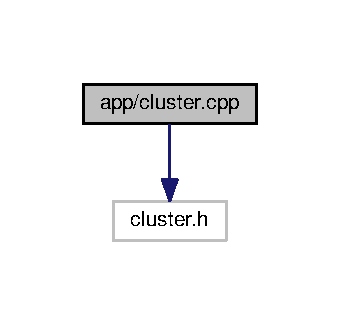
\includegraphics[width=163pt]{cluster_8cpp__incl}
\end{center}
\end{figure}


\subsection{Detailed Description}
$<$\+Implementation file=\char`\"{}\char`\"{} for=\char`\"{}\char`\"{} clustering=\char`\"{}\char`\"{} based=\char`\"{}\char`\"{} on=\char`\"{}\char`\"{} pcl$>$=\char`\"{}\char`\"{}$>$ 

\begin{DoxyAuthor}{Author}
Jerrar Bukhari 
\end{DoxyAuthor}
\begin{DoxyDate}{Date}
15 Oct 2018 
\end{DoxyDate}
\begin{DoxyCopyright}{Copyright}
2018 Jerrar Bukhari 
\end{DoxyCopyright}

\hypertarget{main_8cpp}{}\section{app/main.cpp File Reference}
\label{main_8cpp}\index{app/main.\+cpp@{app/main.\+cpp}}


$<$3D L\+Idar Based Human Detection and localization module$>$  


{\ttfamily \#include $<$main.\+h$>$}\\*
{\ttfamily \#include $<$pcl/common/centroid.\+h$>$}\\*
{\ttfamily \#include $<$iostream$>$}\\*
{\ttfamily \#include $<$vector$>$}\\*
Include dependency graph for main.\+cpp\+:
\nopagebreak
\begin{figure}[H]
\begin{center}
\leavevmode
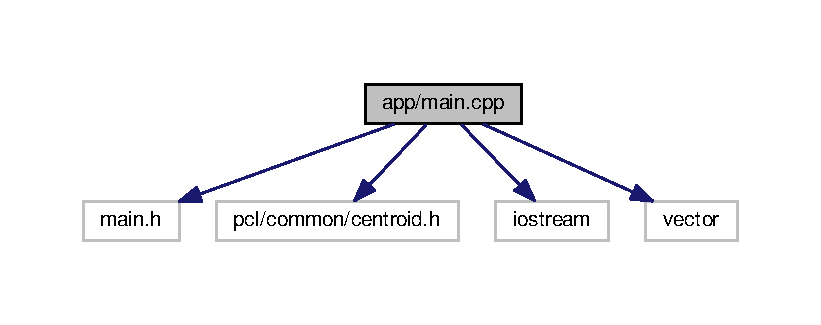
\includegraphics[width=350pt]{main_8cpp__incl}
\end{center}
\end{figure}
\subsection*{Functions}
\begin{DoxyCompactItemize}
\item 
int {\bfseries main} (int argc, char $\ast$$\ast$argv)\hypertarget{main_8cpp_a3c04138a5bfe5d72780bb7e82a18e627}{}\label{main_8cpp_a3c04138a5bfe5d72780bb7e82a18e627}

\item 
void \hyperlink{main_8cpp_a131b249541ea239b1a6b1db058474a77}{visualize} (pcl\+::\+Point\+Cloud$<$ pcl\+::\+Point\+X\+YZ $>$\+::Ptr cloud)
\begin{DoxyCompactList}\small\item\em $<$visualize point=\char`\"{}\char`\"{} cloud=\char`\"{}\char`\"{} data$>$=\char`\"{}\char`\"{}$>$ \end{DoxyCompactList}\item 
void \hyperlink{main_8cpp_ac7f6782c2397b0f552dee6028fb8397a}{visualize} (pcl\+::\+Point\+Cloud$<$ pcl\+::\+Point\+X\+Y\+ZI $>$\+::Ptr cloud)
\begin{DoxyCompactList}\small\item\em $<$visualize point=\char`\"{}\char`\"{} cloud=\char`\"{}\char`\"{} data$>$=\char`\"{}\char`\"{}$>$ \end{DoxyCompactList}\item 
int \hyperlink{main_8cpp_a716cf0cb759cdcee94bc8dbf7878bdfa}{load\+\_\+pcd} (std\+::string filename, pcl\+::\+Point\+Cloud$<$ pcl\+::\+Point\+X\+YZ $>$\+::Ptr cloud)
\begin{DoxyCompactList}\small\item\em $<$load point=\char`\"{}\char`\"{} cloud=\char`\"{}\char`\"{} data$>$=\char`\"{}\char`\"{}$>$ \end{DoxyCompactList}\end{DoxyCompactItemize}


\subsection{Detailed Description}
$<$3D L\+Idar Based Human Detection and localization module$>$ 

\begin{DoxyAuthor}{Author}
Jerrar Bukhari 
\end{DoxyAuthor}
\begin{DoxyDate}{Date}
15 Oct 2018 
\end{DoxyDate}


\subsection{Function Documentation}
\index{main.\+cpp@{main.\+cpp}!load\+\_\+pcd@{load\+\_\+pcd}}
\index{load\+\_\+pcd@{load\+\_\+pcd}!main.\+cpp@{main.\+cpp}}
\subsubsection[{\texorpdfstring{load\+\_\+pcd(std\+::string filename, pcl\+::\+Point\+Cloud$<$ pcl\+::\+Point\+X\+Y\+Z $>$\+::\+Ptr cloud)}{load_pcd(std::string filename, pcl::PointCloud< pcl::PointXYZ >::Ptr cloud)}}]{\setlength{\rightskip}{0pt plus 5cm}int load\+\_\+pcd (
\begin{DoxyParamCaption}
\item[{std\+::string}]{filename, }
\item[{pcl\+::\+Point\+Cloud$<$ pcl\+::\+Point\+X\+YZ $>$\+::Ptr}]{cloud}
\end{DoxyParamCaption}
)}\hypertarget{main_8cpp_a716cf0cb759cdcee94bc8dbf7878bdfa}{}\label{main_8cpp_a716cf0cb759cdcee94bc8dbf7878bdfa}


$<$load point=\char`\"{}\char`\"{} cloud=\char`\"{}\char`\"{} data$>$=\char`\"{}\char`\"{}$>$ 


\begin{DoxyParams}[1]{Parameters}
\mbox{\tt in}  & {\em $<$cloud$>$} & $<$point cloud=\char`\"{}\char`\"{} data=\char`\"{}\char`\"{} holder$>$=\char`\"{}\char`\"{}$>$ \\
\hline
\mbox{\tt in}  & {\em $<$filename$>$} & $<$path to=\char`\"{}\char`\"{} cloud=\char`\"{}\char`\"{} data$>$=\char`\"{}\char`\"{}$>$ \\
\hline
\end{DoxyParams}
\index{main.\+cpp@{main.\+cpp}!visualize@{visualize}}
\index{visualize@{visualize}!main.\+cpp@{main.\+cpp}}
\subsubsection[{\texorpdfstring{visualize(pcl\+::\+Point\+Cloud$<$ pcl\+::\+Point\+X\+Y\+Z $>$\+::\+Ptr cloud)}{visualize(pcl::PointCloud< pcl::PointXYZ >::Ptr cloud)}}]{\setlength{\rightskip}{0pt plus 5cm}void visualize (
\begin{DoxyParamCaption}
\item[{pcl\+::\+Point\+Cloud$<$ pcl\+::\+Point\+X\+YZ $>$\+::Ptr}]{cloud}
\end{DoxyParamCaption}
)}\hypertarget{main_8cpp_a131b249541ea239b1a6b1db058474a77}{}\label{main_8cpp_a131b249541ea239b1a6b1db058474a77}


$<$visualize point=\char`\"{}\char`\"{} cloud=\char`\"{}\char`\"{} data$>$=\char`\"{}\char`\"{}$>$ 


\begin{DoxyParams}[1]{Parameters}
\mbox{\tt in}  & {\em $<$cloud$>$} & $<$point cloud=\char`\"{}\char`\"{} data$>$=\char`\"{}\char`\"{}$>$ \\
\hline
\end{DoxyParams}
\index{main.\+cpp@{main.\+cpp}!visualize@{visualize}}
\index{visualize@{visualize}!main.\+cpp@{main.\+cpp}}
\subsubsection[{\texorpdfstring{visualize(pcl\+::\+Point\+Cloud$<$ pcl\+::\+Point\+X\+Y\+Z\+I $>$\+::\+Ptr cloud)}{visualize(pcl::PointCloud< pcl::PointXYZI >::Ptr cloud)}}]{\setlength{\rightskip}{0pt plus 5cm}void visualize (
\begin{DoxyParamCaption}
\item[{pcl\+::\+Point\+Cloud$<$ pcl\+::\+Point\+X\+Y\+ZI $>$\+::Ptr}]{cloud}
\end{DoxyParamCaption}
)}\hypertarget{main_8cpp_ac7f6782c2397b0f552dee6028fb8397a}{}\label{main_8cpp_ac7f6782c2397b0f552dee6028fb8397a}


$<$visualize point=\char`\"{}\char`\"{} cloud=\char`\"{}\char`\"{} data$>$=\char`\"{}\char`\"{}$>$ 


\begin{DoxyParams}[1]{Parameters}
\mbox{\tt in}  & {\em $<$cloud$>$} & $<$point cloud=\char`\"{}\char`\"{} data$>$=\char`\"{}\char`\"{}$>$ \\
\hline
\end{DoxyParams}

\hypertarget{voxel_8cpp}{}\section{app/voxel.cpp File Reference}
\label{voxel_8cpp}\index{app/voxel.\+cpp@{app/voxel.\+cpp}}


$<$\+Implementation file=\char`\"{}\char`\"{} for=\char`\"{}\char`\"{} voxel=\char`\"{}\char`\"{} grid=\char`\"{}\char`\"{} filter=\char`\"{}\char`\"{} based=\char`\"{}\char`\"{} on=\char`\"{}\char`\"{} pcl$>$=\char`\"{}\char`\"{}$>$  


{\ttfamily \#include $<$voxel.\+h$>$}\\*
Include dependency graph for voxel.\+cpp\+:
\nopagebreak
\begin{figure}[H]
\begin{center}
\leavevmode
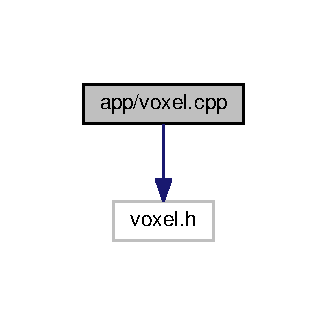
\includegraphics[width=157pt]{voxel_8cpp__incl}
\end{center}
\end{figure}


\subsection{Detailed Description}
$<$\+Implementation file=\char`\"{}\char`\"{} for=\char`\"{}\char`\"{} voxel=\char`\"{}\char`\"{} grid=\char`\"{}\char`\"{} filter=\char`\"{}\char`\"{} based=\char`\"{}\char`\"{} on=\char`\"{}\char`\"{} pcl$>$=\char`\"{}\char`\"{}$>$ 

\begin{DoxyAuthor}{Author}
Jerrar Bukhari 
\end{DoxyAuthor}
\begin{DoxyDate}{Date}
15 Oct 2018 
\end{DoxyDate}
\begin{DoxyCopyright}{Copyright}
2018 Jerrar Bukhari 
\end{DoxyCopyright}

%--- End generated contents ---

% Index
\backmatter
\newpage
\phantomsection
\clearemptydoublepage
\addcontentsline{toc}{chapter}{Index}
\printindex

\end{document}
